\section{Influence Propogation Results}

We ran the independent cascade algorithm on seven randomly generated graphs. The graphs were generated using the scale-free generator, with different parameters passed each time. The values used were as follows:

\begin{table}
\centering
\begin{tabular}{|l|l|}
\hline
Max Neighbours & Scale Factor
\hline
10 & 1
11 & 1.00001
12 & 1.00003
17 & 1.0001
33 & 1.0003
98 & 1.001
279 & 1.003
\hline
\end{tabular}
\caption{Parameters used to generate the scale-free graphs for testing independent cascade.}
\label{tab:ic_graphs}
\end{table}

Each graph contained 10,000 nodes. ``Max neighbours'' is the maximum number of neighbours held by any single node, eg, in the last graph, there exists a node with 279 neighbours. ``Scale factor'' was chosen by trial and error, to ensure that each graph contained 50,000 (+- 500) edges. Each graph had 5 initially converted nodes.

As the average degree distribution was approximately equal for all the graphs, spread of influence through the graph would be more dependent on the network structure.

\ref{tab:ic_results} shows the raw results of this experiment. Note that independent cascade ran iteratively, so the results show the number of converted nodes after each iteration.

\begin{table}
\centering
\begin{tabular}{|l|l|l|}
\hline
Max Neighbours & Iteration & Converted Nodes
\hline
10 & 0 & 5
10 & 1 & 8
10 & 2 & 10
10 & 3 & 10
10 & 4 & 10
\hline
11 & 0 & 5
11 & 1 & 9
11 & 2 & 12
11 & 3 & 13
11 & 4 & 14
11 & 5 & 15
11 & 6 & 15
11 & 7 & 15
\hline
12 & 0 & 5
12 & 1 & 12
12 & 2 & 20
12 & 3 & 26
12 & 4 & 30
12 & 5 & 34
12 & 6 & 37
12 & 7 & 41
12 & 8 & 44
12 & 9 & 50
12 & 10 & 58
12 & 11 & 66
12 & 12 & 71
12 & 13 & 77
12 & 14 & 83
12 & 15 & 87
12 & 16 & 91
12 & 17 & 95
12 & 18 & 96
12 & 19 & 96
12 & 20 & 96
\hline
17 & 0 & 5
17 & 1 & 17
17 & 2 & 31
17 & 3 & 44
17 & 4 & 60
17 & 5 & 75
17 & 6 & 85
17 & 7 & 88
17 & 8 & 90
17 & 9 & 92
17 & 10 & 92
17 & 11 & 92
\hline
33 & 0 & 5
33 & 1 & 10
33 & 2 & 20
33 & 3 & 30
33 & 4 & 40
33 & 5 & 53
33 & 6 & 65
33 & 7 & 84
33 & 8 & 102
33 & 9 & 127
33 & 10 & 162
33 & 11 & 233
33 & 12 & 351
33 & 13 & 489
33 & 14 & 689
33 & 15 & 930
33 & 16 & 1256
33 & 17 & 1627
33 & 18 & 1989
33 & 19 & 2362
33 & 20 & 2697
33 & 21 & 2977
33 & 22 & 3229
33 & 23 & 3422
33 & 24 & 3568
33 & 25 & 3653
33 & 26 & 3704
33 & 27 & 3728
33 & 28 & 3740
33 & 29 & 3748
33 & 30 & 3754
33 & 31 & 3759
33 & 32 & 3764
33 & 33 & 3777
33 & 34 & 3782
33 & 35 & 3789
33 & 36 & 3798
33 & 37 & 3803
33 & 38 & 3805
33 & 39 & 3806
33 & 40 & 3806
33 & 41 & 3806
\hline
98 & 0 & 5
98 & 1 & 17
98 & 2 & 68
98 & 3 & 212
98 & 4 & 729
98 & 5 & 1679
98 & 6 & 2667
98 & 7 & 3048
98 & 8 & 3139
98 & 9 & 3166
98 & 10 & 3166
98 & 11 & 3166
\hline
279 & 0 & 5
279 & 1 & 16
279 & 2 & 205
279 & 3 & 819
279 & 4 & 1762
279 & 5 & 2052
279 & 6 & 2107
279 & 7 & 2107
279 & 8 & 2107
\hline
\end{tabular}
\caption{Independent Cascade: Results.}
\label{tab:ic_results}
\end{table}

\subsection{Graphs}

Each graph plots the number of converted nodes against the number of iterations. Each graph is referred to by it's max neighbours parameter, eg, IC10 refers to the first graph listed in \ref{tab:ic_graphs}.

\begin{figure}[htbp]%
\centering
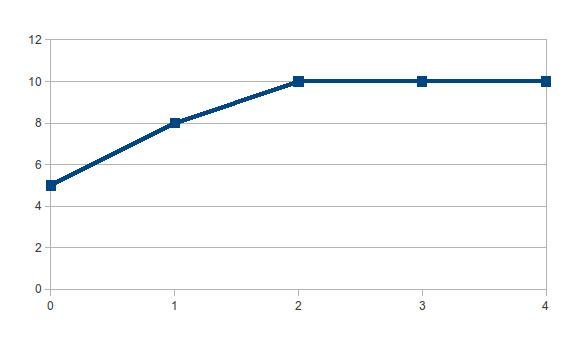
\includegraphics[]{./img/ic10}%
\caption{Spread of influence through IC10}%
\label{fig:ic10}%
\end{figure}

\begin{figure}[htbp]%
\centering
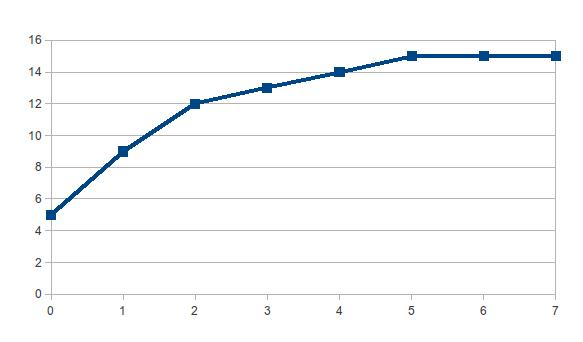
\includegraphics[]{./img/ic11}%
\caption{Spread of influence through IC11}%
\label{fig:ic11}%
\end{figure}

\begin{figure}[htbp]%
\centering
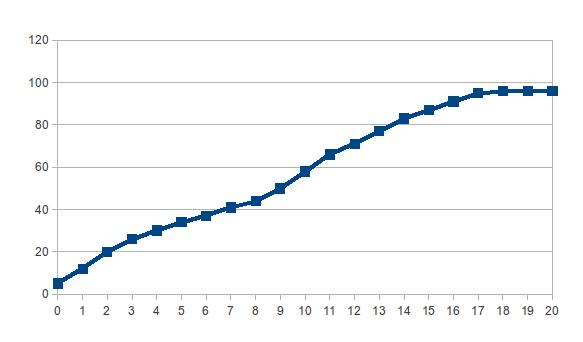
\includegraphics[]{./img/ic12}%
\caption{Spread of influence through IC12}%
\label{fig:ic12}%
\end{figure}

\begin{figure}[htbp]%
\centering
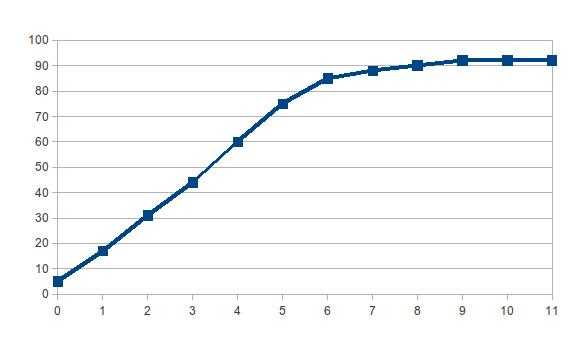
\includegraphics[]{./img/ic17}%
\caption{Spread of influence through IC17}%
\label{fig:ic17}%
\end{figure}

\begin{figure}[htbp]%
\centering
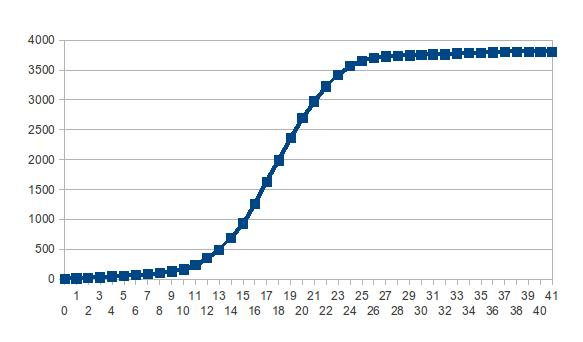
\includegraphics[]{./img/ic33}%
\caption{Spread of influence through IC33}%
\label{fig:ic33}%
\end{figure}

\begin{figure}[htbp]%
\centering
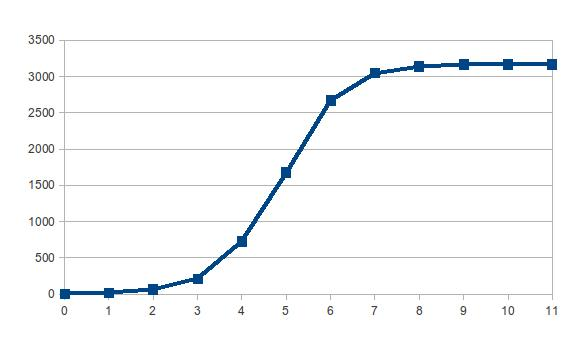
\includegraphics[]{./img/ic98}%
\caption{Spread of influence through IC98}%
\label{fig:ic98}%
\end{figure}

\begin{figure}[htbp]%
\centering
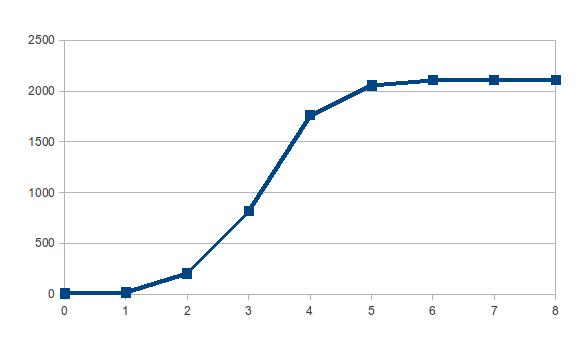
\includegraphics[]{./img/ic279}%
\caption{Spread of influence through IC279}%
\label{fig:ic10}%
\end{figure}

\subsection{Conclusions}

Graphs IC10, IC11, IC12 and IC17 exhibit very small influence cascades, of less than 100 nodes each, although they do show a steady increade in influence cascade size. Between IC17 and IC33, a tipping point is reached, and the cascade in IC33 covers over one third of the graph. The cascade of IC98 covers roughly the same area, but reached this point much more quickly. IC279 is also large, though smaller than IC33 and IC98.

In the above experiment, edges had a roughly 10\% chance of remaining live (live edges are those that represent sucessful conversion attempts), so nodes in all the graphs would have had an average of 1 convertable neighbour. However, the variance would have been much higher in the graphs IC33-279, so some nodes in these graphs would have had many live neighbours. In the graphs IC10-17, in contrast, almost all the nodes would have had a very low number of neighbours.

This explains why the early graphs show such small influence cascades -- as almost all nodes will have a low number of live edges, cascades ``fizzle out'' quickly. In the later graphs, there will be many nodes with 1 or 0 live edges, but a minority of nodes with many live edges. It is these nodes that allow cascades in these graphs to spread so far. We can also see that the 3 graphs IC33-279 show a clear sigmoid curve shape. This suggests that cascades in these graphs followed a slow initial growth, followed by a conversion of several ``hub'' nodes and a rapid take-off, and finally a slowdown as the cascade hits natural limits.

The fact that the IC279 cascade is smaller than IC33 and IC98 might be due to random factors, or it might suggest that influence is less likely to spread through heavily skewed graphs, as a majority of nodes will end up with no live edges.

\subsection{Extensions}

Several interesting avenues of exploration were not possible due to time constraints. 
As the experiments above had a strong random element, running multiple trials -- ie, Monte Carlo simulations -- would provide more accurate results.

Running experiments on the Linear Threshold model would be another obvious avenue for exploration.

Many papers looked at how the distribution of influence probabilities affected the spread of influence. In the above experiments, influence weights were chosen uniformly in the range (0,0.2), meaning that approximately 10\% of the edges in a given graph would be ``live''. Using a wider or narrower range of probabilities, or a different probability distribution, would likely have a strong effect on the final spread of the cascade.


